%#########################1########################

 \cajita{%
Asignación presupuestaria a la SESAN }%
{%
	La SESAN es la Secretaría de Seguridad Alimentaria y Nutricional de la presidencia de la república. Es importante conocer el porcentaje de asignación que se hace a esta secretaria respecto al presupuesto de ingresos e ingresos de la nación. En 2015 está asignación fue del 7.7\%\footnote{La asignación presupuestaria no siempre logra ser ejecutada en su totalidad por las instituciones de gobierno}.  
 }%
{%
 Tasa de asignación presupuestaria a la SESAN respecto del presupuesto general de la nación } %
{%
 República de Guatemala, serie histórica, en porcentaje} %
{%
 \begin{tikzpicture}[x=1pt,y=1pt]  % Created by tikzDevice version 0.9 on 2016-03-03 06:36:56
% !TEX encoding = UTF-8 Unicode
\definecolor{fillColor}{RGB}{255,255,255}
\path[use as bounding box,fill=fillColor,fill opacity=0.00] (0,0) rectangle (289.08,198.74);
\begin{scope}
\path[clip] (  0.00,  0.00) rectangle (289.08,198.74);

\path[] (  0.00,  0.00) rectangle (289.08,198.74);
\end{scope}
\begin{scope}
\path[clip] (  0.00,  0.00) rectangle (289.08,198.74);

\path[] (  1.74, 15.61) rectangle (280.54,191.48);

\path[] (  1.74, 37.77) --
	(280.54, 37.77);

\path[] (  1.74, 86.42) --
	(280.54, 86.42);

\path[] (  1.74,135.08) --
	(280.54,135.08);

\path[] (  1.74,183.73) --
	(280.54,183.73);

\path[] (  1.74, 62.10) --
	(280.54, 62.10);

\path[] (  1.74,110.75) --
	(280.54,110.75);

\path[] (  1.74,159.40) --
	(280.54,159.40);

\path[] ( 54.01, 15.61) --
	( 54.01,191.48);

\path[] (141.14, 15.61) --
	(141.14,191.48);

\path[] (228.27, 15.61) --
	(228.27,191.48);
\definecolor{drawColor}{RGB}{0,0,255}

\path[draw=drawColor,line width= 1.7pt,line join=round] ( 54.01,183.49) --
	(141.14,144.70) --
	(228.27, 60.50);
\definecolor{drawColor}{RGB}{0,0,0}

\node[text=drawColor,anchor=base,inner sep=0pt, outer sep=0pt, scale=  1.02] at ( 54.01,187.46) {7.9};

\node[text=drawColor,anchor=base west,inner sep=0pt, outer sep=0pt, scale=  1.02] at (141.14,148.68) {7.9};

\node[text=drawColor,anchor=base,inner sep=0pt, outer sep=0pt, scale=  1.02] at (228.27, 48.59) {7.7};

\path[draw=drawColor,line width= 0.1pt,line join=round] (  1.74, 23.61) -- (280.54, 23.61);

\path[] (  1.74, 15.61) rectangle (280.54,191.48);
\end{scope}
\begin{scope}
\path[clip] (  0.00,  0.00) rectangle (289.08,198.74);

\path[] (  1.74, 15.61) --
	(  1.74,191.48);
\end{scope}
\begin{scope}
\path[clip] (  0.00,  0.00) rectangle (289.08,198.74);

\path[] (  0.00, 62.10) --
	(  1.74, 62.10);

\path[] (  0.00,110.75) --
	(  1.74,110.75);

\path[] (  0.00,159.40) --
	(  1.74,159.40);
\end{scope}
\begin{scope}
\path[clip] (  0.00,  0.00) rectangle (289.08,198.74);

\path[] (  1.74, 15.61) --
	(280.54, 15.61);
\end{scope}
\begin{scope}
\path[clip] (  0.00,  0.00) rectangle (289.08,198.74);

\path[] ( 54.01, 12.86) --
	( 54.01, 15.61);

\path[] (141.14, 12.86) --
	(141.14, 15.61);

\path[] (228.27, 12.86) --
	(228.27, 15.61);
\end{scope}
\begin{scope}
\path[clip] (  0.00,  0.00) rectangle (289.08,198.74);
\definecolor{drawColor}{RGB}{0,0,0}

\node[text=drawColor,anchor=base,inner sep=0pt, outer sep=0pt, scale=  1.00] at ( 54.01,  2.85) {2012};

\node[text=drawColor,anchor=base,inner sep=0pt, outer sep=0pt, scale=  1.00] at (141.14,  2.85) {2014};

\node[text=drawColor,anchor=base,inner sep=0pt, outer sep=0pt, scale=  1.00] at (228.27,  2.85) {2015};
\end{scope}
  \end{tikzpicture}}%
{%
 SICOIN} %


 \cajita{%
 	Ejecución presupuestaria de la SESAN }%
 {%
 	El porcentaje de ejecución presupuestaria es la razón entre el monto total erogado por la SESAN respecto de su asignación presupuestaria. 
 	
 	La ejecución presupuestaria de la SESAN entre el 2012 y 2015 ha variado entre 66.6 y 89.2 por ciento, teniendo su ejecuación más baja en el 2015.
 }%
 {%
 	Tasa de ejecución de la SESAN respecto al presupuesto asignado } %
 {%
 	República de Guatemala, serie histórica, en porcentaje} %
 {%
 	\begin{tikzpicture}[x=1pt,y=1pt]  % Created by tikzDevice version 0.9 on 2016-03-03 06:36:58
% !TEX encoding = UTF-8 Unicode
\definecolor{fillColor}{RGB}{255,255,255}
\path[use as bounding box,fill=fillColor,fill opacity=0.00] (0,0) rectangle (289.08,198.74);
\begin{scope}
\path[clip] (  0.00,  0.00) rectangle (289.08,198.74);

\path[] (  0.00,  0.00) rectangle (289.08,198.74);
\end{scope}
\begin{scope}
\path[clip] (  0.00,  0.00) rectangle (289.08,198.74);

\path[] ( -0.52, 15.61) rectangle (280.54,191.48);

\path[] (  0.00, 51.79) --
	(280.54, 51.79);

\path[] (  0.00,106.22) --
	(280.54,106.22);

\path[] (  0.00,160.66) --
	(280.54,160.66);

\path[] (  0.00, 24.58) --
	(280.54, 24.58);

\path[] (  0.00, 79.01) --
	(280.54, 79.01);

\path[] (  0.00,133.44) --
	(280.54,133.44);

\path[] (  0.00,187.87) --
	(280.54,187.87);

\path[] ( 39.63, 15.61) --
	( 39.63,191.48);

\path[] (106.55, 15.61) --
	(106.55,191.48);

\path[] (173.47, 15.61) --
	(173.47,191.48);

\path[] (240.39, 15.61) --
	(240.39,191.48);
\definecolor{drawColor}{RGB}{0,0,255}

\path[draw=drawColor,line width= 1.7pt,line join=round] ( 39.63,183.49) --
	(106.55,106.32) --
	(173.47,161.99) --
	(240.39, 60.50);
\definecolor{drawColor}{RGB}{0,0,0}

\node[text=drawColor,anchor=base,inner sep=0pt, outer sep=0pt, scale=  1.02] at ( 39.63,187.46) {89.2};

\node[text=drawColor,anchor=base,inner sep=0pt, outer sep=0pt, scale=  1.02] at (106.55, 94.41) {75.0};

\node[text=drawColor,anchor=base,inner sep=0pt, outer sep=0pt, scale=  1.02] at (173.47,165.96) {85.2};

\node[text=drawColor,anchor=base,inner sep=0pt, outer sep=0pt, scale=  1.02] at (240.39, 48.59) {66.6};

\path[draw=drawColor,line width= 0.1pt,line join=round] (  0.00, 23.61) -- (280.54, 23.61);

\path[] ( -0.52, 15.61) rectangle (280.54,191.48);
\end{scope}
\begin{scope}
\path[clip] (  0.00,  0.00) rectangle (289.08,198.74);

\path[] (  0.00, 15.61) --
	(280.54, 15.61);
\end{scope}
\begin{scope}
\path[clip] (  0.00,  0.00) rectangle (289.08,198.74);

\path[] ( 39.63, 12.86) --
	( 39.63, 15.61);

\path[] (106.55, 12.86) --
	(106.55, 15.61);

\path[] (173.47, 12.86) --
	(173.47, 15.61);

\path[] (240.39, 12.86) --
	(240.39, 15.61);
\end{scope}
\begin{scope}
\path[clip] (  0.00,  0.00) rectangle (289.08,198.74);
\definecolor{drawColor}{RGB}{0,0,0}

\node[text=drawColor,anchor=base,inner sep=0pt, outer sep=0pt, scale=  1.00] at ( 39.63,  2.85) {2012};

\node[text=drawColor,anchor=base,inner sep=0pt, outer sep=0pt, scale=  1.00] at (106.55,  2.85) {2013};

\node[text=drawColor,anchor=base,inner sep=0pt, outer sep=0pt, scale=  1.00] at (173.47,  2.85) {2014};

\node[text=drawColor,anchor=base,inner sep=0pt, outer sep=0pt, scale=  1.00] at (240.39,  2.85) {2015};
\end{scope}
  \end{tikzpicture}}%
 {%
 	SICOIN} %
 
 
  \cajita{%
  	Detalle de gasto de la SESAN }%
  {%
  	Para atender la desnutrición se implementó el plan hambre cero\footnote{El Plan hambre cero representa una estrategia conjunta de atención a la desnutrición crónica, la
  		desnutrición aguda y la inseguridad alimentaria, que afectan principalmente a la niñez
  		guatemalteca menor de cinco años, que vive en condiciones de pobreza y pobreza
  		extrema. Está focalizado especialmente en el área rural y urbana marginal del país, y
  		promueve la creación de condiciones y medios necesarios para la generación en el
  		mediano y largo plazo, de una seguridad alimentaria y nutricional efectiva y sostenible,
  		con el propósito de disminuir en forma significativa la desnutrición crónica y la
  		desnutrición aguda que afecta a la niñez guatemalteca.
  		}, siendo la SESAN parte importante en la ejecución del mismo. 
  		
  		En Plan Hambre Cero está compuesto por componentes directos, de viabilidad y el eje transversal\footnote{La transversalidad se refiere a aquellos temas cuyo contenido debe ser aplicado en
  			forma intrínseca, integral y apropiada en todos los componente del Plan Hambre Cero.
  			}, siendo este último el aspecto en la que más se invirtió dinero por parte de la SESAN para el 2015
  	
  	
  }%
  {%
  	Detalle de ejecución de la SESAN } %
  {%
  	República de Guatemala, 2014, en quetzales} %
  {%
  	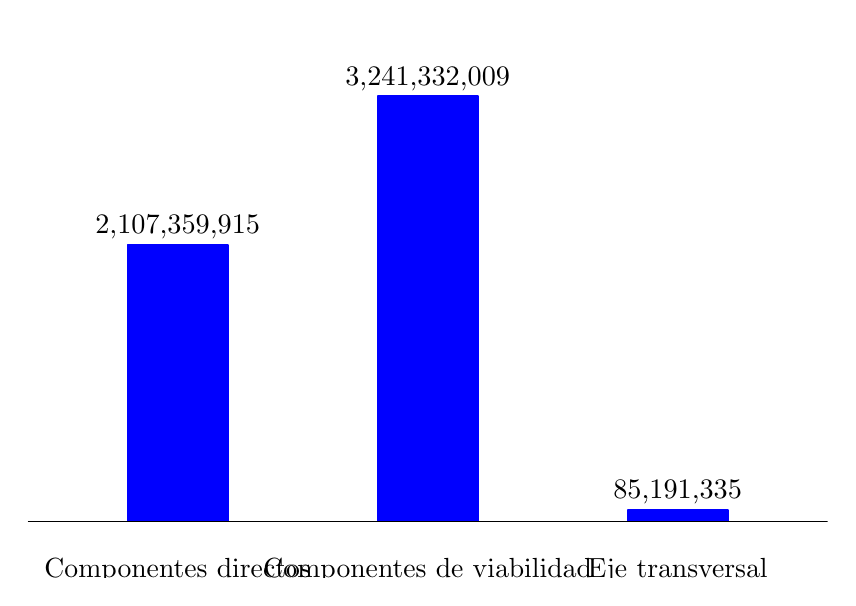
\begin{tikzpicture}[x=1pt,y=1pt]  % Created by tikzDevice version 0.9 on 2016-03-03 06:36:59
% !TEX encoding = UTF-8 Unicode
\definecolor{fillColor}{RGB}{255,255,255}
\path[use as bounding box,fill=fillColor,fill opacity=0.00] (0,0) rectangle (289.08,198.74);
\begin{scope}
\path[clip] (  0.00,  0.00) rectangle (289.08,198.74);

\path[] (  0.00,  0.00) rectangle (289.08,198.74);
\end{scope}
\begin{scope}
\path[clip] (  0.00,  0.00) rectangle (289.08,198.74);

\path[] (  0.00, 12.77) rectangle (289.08,181.67);

\path[] ( 54.20, 12.77) --
	( 54.20,181.67);

\path[] (144.54, 12.77) --
	(144.54,181.67);

\path[] (234.88, 12.77) --
	(234.88,181.67);
\definecolor{drawColor}{RGB}{0,0,255}
\definecolor{fillColor}{RGB}{0,0,255}

\path[draw=drawColor,line width= 0.6pt,line join=round,fill=fillColor] ( 36.13, 20.44) rectangle ( 72.27,120.27);

\path[draw=drawColor,line width= 0.6pt,line join=round,fill=fillColor] (126.47, 20.44) rectangle (162.61,173.99);

\path[draw=drawColor,line width= 0.6pt,line join=round,fill=fillColor] (216.81, 20.44) rectangle (252.95, 24.48);
\definecolor{drawColor}{RGB}{0,0,0}

\path[draw=drawColor,line width= 0.1pt,line join=round] (  0.00, 20.44) -- (289.08, 20.44);

\node[text=drawColor,anchor=base,inner sep=0pt, outer sep=0pt, scale=  1.02] at ( 54.20,124.25) {2,107,359,915};

\node[text=drawColor,anchor=base,inner sep=0pt, outer sep=0pt, scale=  1.02] at (144.54,177.96) {3,241,332,009};

\node[text=drawColor,anchor=base,inner sep=0pt, outer sep=0pt, scale=  1.02] at (234.88, 28.45) {85,191,335};

\path[] (  0.00, 12.77) rectangle (289.08,181.67);
\end{scope}
\begin{scope}
\path[clip] (  0.00,  0.00) rectangle (289.08,198.74);

\path[] (  0.00, 12.77) --
	(289.08, 12.77);
\end{scope}
\begin{scope}
\path[clip] (  0.00,  0.00) rectangle (289.08,198.74);

\path[] ( 54.20, 10.02) --
	( 54.20, 12.77);

\path[] (144.54, 10.02) --
	(144.54, 12.77);

\path[] (234.88, 10.02) --
	(234.88, 12.77);
\end{scope}
\begin{scope}
\path[clip] (  0.00,  0.00) rectangle (289.08,198.74);
\definecolor{drawColor}{RGB}{0,0,0}

\node[text=drawColor,anchor=base,inner sep=0pt, outer sep=0pt, scale=  1.00] at ( 54.20, -0.00) {Componentes directos};

\node[text=drawColor,anchor=base,inner sep=0pt, outer sep=0pt, scale=  1.00] at (144.54, -0.00) {Componentes de viabilidad};

\node[text=drawColor,anchor=base,inner sep=0pt, outer sep=0pt, scale=  1.00] at (234.88, -0.00) {Eje transversal};
\end{scope}
  \end{tikzpicture}}%
  {%
  	SICOIN} %
  
  
  
  \cajita{%
  	Asignación presupuestaria a la ventana de los mil días}%
  {%
  	La ventana de los mil días\footnote{es el período que transcurre desde el embarazo -270 días promedio- hasta los dos años de vida del niño -730 días- } es una estrategia lanzada por el Ministerio de Salud Pública y Asistencia Social y funciona como un paquete de atención en salud y nutrición cuyo objetivo principal es reducir y prevenir la desnutrición crónica en Guatemala
  	
  	En la serie histórica se observa que ha habido un aumento en la inversión para el plan la ventana de los mil días. En el 2015 se hizo una asignación de 705,840,558 quetzales. 
  }%
  {%
  Asignación presupuestaria al programa ventana de los mi días para el año 2015} %
  {%
  	República de Guatemala, serie histórica, en quetzales} %
  {%
  	\begin{tikzpicture}[x=1pt,y=1pt]  % Created by tikzDevice version 0.9 on 2016-03-03 06:37:00
% !TEX encoding = UTF-8 Unicode
\definecolor{fillColor}{RGB}{255,255,255}
\path[use as bounding box,fill=fillColor,fill opacity=0.00] (0,0) rectangle (289.08,198.74);
\begin{scope}
\path[clip] (  0.00,  0.00) rectangle (289.08,198.74);

\path[] (  0.00,  0.00) rectangle (289.08,198.74);
\end{scope}
\begin{scope}
\path[clip] (  0.00,  0.00) rectangle (289.08,198.74);

\path[] ( 12.53, 15.61) rectangle (280.54,191.48);

\path[] ( 12.53, 54.04) --
	(280.54, 54.04);

\path[] ( 12.53, 96.77) --
	(280.54, 96.77);

\path[] ( 12.53,139.51) --
	(280.54,139.51);

\path[] ( 12.53,182.24) --
	(280.54,182.24);

\path[] ( 12.53, 32.67) --
	(280.54, 32.67);

\path[] ( 12.53, 75.41) --
	(280.54, 75.41);

\path[] ( 12.53,118.14) --
	(280.54,118.14);

\path[] ( 12.53,160.87) --
	(280.54,160.87);

\path[] ( 62.78, 15.61) --
	( 62.78,191.48);

\path[] (146.54, 15.61) --
	(146.54,191.48);

\path[] (230.29, 15.61) --
	(230.29,191.48);
\definecolor{drawColor}{RGB}{0,0,255}

\path[draw=drawColor,line width= 1.7pt,line join=round] ( 62.78, 60.50) --
	(146.54,113.90) --
	(230.29,183.49);
\definecolor{drawColor}{RGB}{0,0,0}

\node[text=drawColor,anchor=base,inner sep=0pt, outer sep=0pt, scale=  1.02] at ( 62.78, 48.59) {130,246,108};

\node[text=drawColor,anchor=base east,inner sep=0pt, outer sep=0pt, scale=  1.02] at (137.61,113.90) {380,172,611};

\node[text=drawColor,anchor=base,inner sep=0pt, outer sep=0pt, scale=  1.02] at (230.29,187.46) {705,840,558};

\path[draw=drawColor,line width= 0.1pt,line join=round] ( 12.53, 23.61) -- (280.54, 23.61);

\path[] ( 12.53, 15.61) rectangle (280.54,191.48);
\end{scope}
\begin{scope}
\path[clip] (  0.00,  0.00) rectangle (289.08,198.74);

\path[] ( 12.53, 15.61) --
	( 12.53,191.48);
\end{scope}
\begin{scope}
\path[clip] (  0.00,  0.00) rectangle (289.08,198.74);
\definecolor{drawColor}{RGB}{255,255,255}

\node[text=drawColor,text opacity=0.00,anchor=base east,inner sep=0pt, outer sep=0pt, scale=  1.00] at (  7.58, 28.76) {0e+00};

\node[text=drawColor,text opacity=0.00,anchor=base east,inner sep=0pt, outer sep=0pt, scale=  1.00] at (  7.58, 71.50) {2e+08};

\node[text=drawColor,text opacity=0.00,anchor=base east,inner sep=0pt, outer sep=0pt, scale=  1.00] at (  7.58,114.23) {4e+08};

\node[text=drawColor,text opacity=0.00,anchor=base east,inner sep=0pt, outer sep=0pt, scale=  1.00] at (  7.58,156.97) {6e+08};
\end{scope}
\begin{scope}
\path[clip] (  0.00,  0.00) rectangle (289.08,198.74);

\path[] (  9.78, 32.67) --
	( 12.53, 32.67);

\path[] (  9.78, 75.41) --
	( 12.53, 75.41);

\path[] (  9.78,118.14) --
	( 12.53,118.14);

\path[] (  9.78,160.87) --
	( 12.53,160.87);
\end{scope}
\begin{scope}
\path[clip] (  0.00,  0.00) rectangle (289.08,198.74);

\path[] ( 12.53, 15.61) --
	(280.54, 15.61);
\end{scope}
\begin{scope}
\path[clip] (  0.00,  0.00) rectangle (289.08,198.74);

\path[] ( 62.78, 12.86) --
	( 62.78, 15.61);

\path[] (146.54, 12.86) --
	(146.54, 15.61);

\path[] (230.29, 12.86) --
	(230.29, 15.61);
\end{scope}
\begin{scope}
\path[clip] (  0.00,  0.00) rectangle (289.08,198.74);
\definecolor{drawColor}{RGB}{0,0,0}

\node[text=drawColor,anchor=base,inner sep=0pt, outer sep=0pt, scale=  1.00] at ( 62.78,  2.85) {2013};

\node[text=drawColor,anchor=base,inner sep=0pt, outer sep=0pt, scale=  1.00] at (146.54,  2.85) {2014};

\node[text=drawColor,anchor=base,inner sep=0pt, outer sep=0pt, scale=  1.00] at (230.29,  2.85) {2015};
\end{scope}
  \end{tikzpicture}}%
  {%
  	SICOIN} %
  
  
    \cajita{%
    	Gasto programa ventana de los mil días}%
    {%
    	El programa la ventana de los mil días tiene varios rubros de inversión, que responden a necesidades que la población necesita satisfacer.
    	
    	Para el 2015 el gasto se centralizó en la compra de vacunas, seguido de la compra de Vitamina A.
    }%
    {%
    	Detalle del gasto en el programa ventana de los mil días} %
    {%
    	República de Guatemala, 2015, en miles de millones quetzales} %
    {%
    	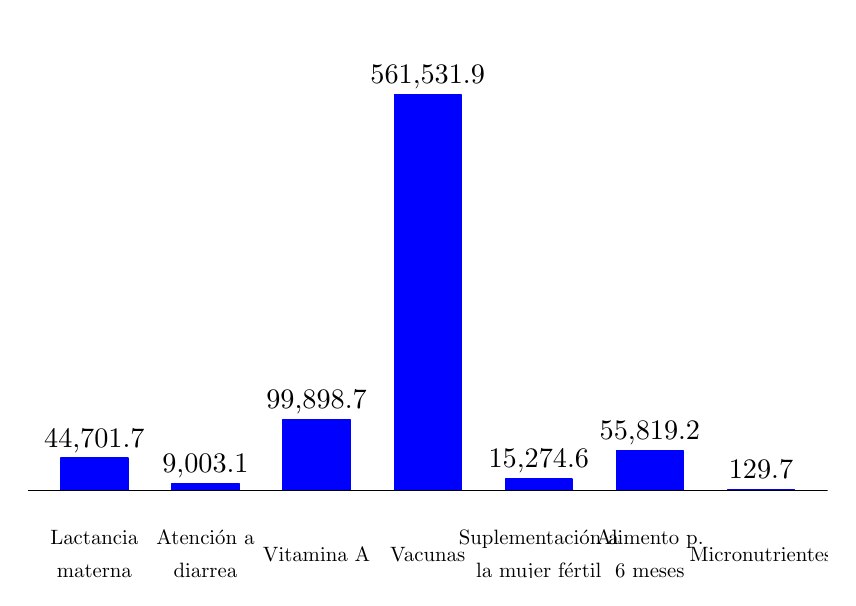
\begin{tikzpicture}[x=1pt,y=1pt]  % Created by tikzDevice version 0.9 on 2016-03-03 06:46:08
% !TEX encoding = UTF-8 Unicode
\definecolor{fillColor}{RGB}{255,255,255}
\path[use as bounding box,fill=fillColor,fill opacity=0.00] (0,0) rectangle (289.08,198.74);
\begin{scope}
\path[clip] (  0.00,  0.00) rectangle (289.08,198.74);

\path[] (  0.00,  0.00) rectangle (289.08,198.74);
\end{scope}
\begin{scope}
\path[clip] (  0.00,  0.00) rectangle (289.08,198.74);

\path[] (  0.00, 24.65) rectangle (289.08,181.67);

\path[] ( 24.09, 24.65) --
	( 24.09,181.67);

\path[] ( 64.24, 24.65) --
	( 64.24,181.67);

\path[] (104.39, 24.65) --
	(104.39,181.67);

\path[] (144.54, 24.65) --
	(144.54,181.67);

\path[] (184.69, 24.65) --
	(184.69,181.67);

\path[] (224.84, 24.65) --
	(224.84,181.67);

\path[] (264.99, 24.65) --
	(264.99,181.67);
\definecolor{drawColor}{RGB}{0,0,255}
\definecolor{fillColor}{RGB}{0,0,255}

\path[draw=drawColor,line width= 0.6pt,line join=round,fill=fillColor] ( 12.04, 31.78) rectangle ( 36.14, 43.15);

\path[draw=drawColor,line width= 0.6pt,line join=round,fill=fillColor] ( 52.20, 31.78) rectangle ( 76.29, 34.07);

\path[draw=drawColor,line width= 0.6pt,line join=round,fill=fillColor] ( 92.35, 31.78) rectangle (116.43, 57.18);

\path[draw=drawColor,line width= 0.6pt,line join=round,fill=fillColor] (132.50, 31.78) rectangle (156.59,174.53);

\path[draw=drawColor,line width= 0.6pt,line join=round,fill=fillColor] (172.64, 31.78) rectangle (196.73, 35.67);

\path[draw=drawColor,line width= 0.6pt,line join=round,fill=fillColor] (212.80, 31.78) rectangle (236.88, 45.97);

\path[draw=drawColor,line width= 0.6pt,line join=round,fill=fillColor] (252.94, 31.78) rectangle (277.03, 31.82);
\definecolor{drawColor}{RGB}{0,0,0}

\path[draw=drawColor,line width= 0.1pt,line join=round] (  0.00, 31.78) -- (289.08, 31.78);

\node[text=drawColor,anchor=base,inner sep=0pt, outer sep=0pt, scale=  1.02] at ( 24.09, 47.12) {44,701.7};

\node[text=drawColor,anchor=base,inner sep=0pt, outer sep=0pt, scale=  1.02] at ( 64.24, 38.04) {9,003.1};

\node[text=drawColor,anchor=base,inner sep=0pt, outer sep=0pt, scale=  1.02] at (104.39, 61.15) {99,898.7};

\node[text=drawColor,anchor=base,inner sep=0pt, outer sep=0pt, scale=  1.02] at (144.54,178.50) {561,531.9};

\node[text=drawColor,anchor=base,inner sep=0pt, outer sep=0pt, scale=  1.02] at (184.69, 39.64) {15,274.6};

\node[text=drawColor,anchor=base,inner sep=0pt, outer sep=0pt, scale=  1.02] at (224.84, 49.95) {55,819.2};

\node[text=drawColor,anchor=base,inner sep=0pt, outer sep=0pt, scale=  1.02] at (264.99, 35.79) {129.7};

\path[] (  0.00, 24.65) rectangle (289.08,181.67);
\end{scope}
\begin{scope}
\path[clip] (  0.00,  0.00) rectangle (289.08,198.74);

\path[] (  0.00, 24.65) --
	(289.08, 24.65);
\end{scope}
\begin{scope}
\path[clip] (  0.00,  0.00) rectangle (289.08,198.74);

\path[] ( 24.09, 21.90) --
	( 24.09, 24.65);

\path[] ( 64.24, 21.90) --
	( 64.24, 24.65);

\path[] (104.39, 21.90) --
	(104.39, 24.65);

\path[] (144.54, 21.90) --
	(144.54, 24.65);

\path[] (184.69, 21.90) --
	(184.69, 24.65);

\path[] (224.84, 21.90) --
	(224.84, 24.65);

\path[] (264.99, 21.90) --
	(264.99, 24.65);
\end{scope}
\begin{scope}
\path[clip] (  0.00,  0.00) rectangle (289.08,198.74);
\definecolor{drawColor}{RGB}{0,0,0}

\node[text=drawColor,anchor=base,inner sep=0pt, outer sep=0pt, scale=  0.750] at ( 24.09, 11.88) {Lactancia };

\node[text=drawColor,anchor=base,inner sep=0pt, outer sep=0pt, scale=  0.750] at ( 24.09,  0.00) {  materna};

\node[text=drawColor,anchor=base,inner sep=0pt, outer sep=0pt, scale=  0.750] at ( 64.24, 11.88) {Atención a };

\node[text=drawColor,anchor=base,inner sep=0pt, outer sep=0pt, scale=  0.750] at ( 64.24,  0.00) { diarrea};

\node[text=drawColor,anchor=base,inner sep=0pt, outer sep=0pt, scale=  0.750] at (104.39,  5.94) {Vitamina A};

\node[text=drawColor,anchor=base,inner sep=0pt, outer sep=0pt, scale=  0.750] at (144.54,  5.94) {Vacunas};

\node[text=drawColor,anchor=base,inner sep=0pt, outer sep=0pt, scale=  0.750] at (184.69, 11.88) {Suplementación a };

\node[text=drawColor,anchor=base,inner sep=0pt, outer sep=0pt, scale=  0.750] at (184.69,  0.00) { la mujer fértil};

\node[text=drawColor,anchor=base,inner sep=0pt, outer sep=0pt, scale=  0.750] at (224.84, 11.88) {Alimento p. };

\node[text=drawColor,anchor=base,inner sep=0pt, outer sep=0pt, scale=  0.750] at (224.84,  0.00) { 6 meses};

\node[text=drawColor,anchor=base,inner sep=0pt, outer sep=0pt, scale=  0.750] at (264.99,  5.94) {Micronutrientes};
\end{scope}
  \end{tikzpicture}}%
    {%
    	SICOIN} %
  